\chapter{Implementacja}
\section{Wprowadzenie}
Celem tego rozdziału jest szczegółowy opis podejścia do realizacji projektu BBS, a mianowicie wyjaśnienie podstawowych pojęć, analiza architektury oraz algorytmów stosowanych do przetwarzania danych.

Chciałbym zacząć od tego, czym właściwie jest BBS. Zgodnie z definicją projekt jest w rzeczywistości procesorem języka \cite{compilers}, a konkretnie tłumaczem według następujących cech, które wynikają bezpośrednio z wymagań opisanych w sekcji 2:
\begin{itemize}
    \item Oprogramowanie analizuje kod wejściowy, napisany w specjalnie opracowanym na potrzeby projektu języku
    \item Oprogramowanie powinno wykrywać i raportować możliwe błędy logiczne lub składniowe w pliku wejściowym
    \item Zamiast tłumaczyć plik wejściowy na inny język programowania, program powinien wykonać polecenia opisane w pliku wejściowym
\end{itemize}

Dodatkowo oprogramowanie to zawiera również preprocesor. Dzieje się tak, aby plik wejściowy mógł zostać podzielony na wiele części, co umożliwi działanie mechanizmu budowania podprojektu.

\section{Gramatyka języka}

W tej sekcji wprowadzimy notację -- ''gramatykę bezkontekstową'' lub dla zwięzłości ''gramatykę'' -- która jest używana do definiowania składni języka. Gramatyka będzie używana w tej książce do organizowania interfejsu kompilatora. Gramatyka w naturalny sposób opisuje hierarchiczną strukturę większości struktur językowych \cite{compilers}. Używając zmiennej \texttt{expr} do oznaczenia wyrażenia i zmiennej \texttt{stmt} do oznaczenia instrukcji, tę regułę strukturyzacji można wyrazić jako :

\begin{lstlisting}[label=list:example_grammar,caption=Przykładowy opis gramatyki,basicstyle=\footnotesize\ttfamily]
stmt -> if (expr) stmt else stmt
\end{lstlisting}

w którą strzałkę można odczytać jako „może mieć formę”. Taka zasada nazywa się ''produkcją''. Produkty posiadają takie elementy leksykalne, jak słowo kluczowe \texttt{if} i nawias, nazywane są ''terminalami''. Zmienne takie jak \texttt{expr} i \texttt{stmt} reprezentują sekwencje terminali i nazywane są ''nieterminalami''.

Gramatyka bezkontekstowa składa się z czterech elementów:
\begin{itemize}
    \item Zestaw znaków końcowych, czasami nazywany „tokenami”. Terminale to podstawowe symbole języka zdefiniowane przez gramatykę.
    \item Zbiór nieterminali, czasami nazywany „zmiennymi składniowymi”. Każdy nieterminal reprezentuje zestaw ciągów końcowych, tak jak to zrobimy opisać
    \item Zbiór produkcji, gdzie każda produkcja składa się z nieterminala, zwanego głową lub lewą stroną produkcji, strzałki oraz sekwencji terminali i nieterminali, zwanej treścią lub prawą stroną produkcji.
    \item Oznaczenie jednego z nieterminali jako symbolu początkowego.
\end{itemize}

\subsection{Gramatyka języka BBS}

Główne wymagania stawiane językowi stosowanemu w projekcie BBS to prostota gramatyki, minimalna liczba słów kluczowych, typów danych i zmiennych wewnętrznych. W trakcie pracy powstał język o następującej gramatyce:

\begin{lstlisting}[label=list:grammar,caption=Gramatyka języka projektu BBS,basicstyle=\footnotesize\ttfamily]
script -> declarations statements
statements -> statements statement | epsilon
statement -> !prj string | !files array | 
			 !deps array | !cflags string | 
			 !pre string | !post string | 
			 !inc array

declarations -> declarations declaration | epsilon
declaration -> !let id = string

array -> [ strings variables ]
strings -> strings, string | epsilon
variables -> variables, variable | epsilon

string -> "characters separators punctuators"
variable -> $id
id -> characters

characters -> characters character | epsilon
character -> A | B |..| z
separators -> separators separator | epsilon
separator -> SPACE
punctuators -> punctuators punctuator | epsilon
punctuator -> / | - | _ | . | ,
\end{lstlisting}

Jak widać z opisu gramatyki, język operuje na dwóch głównych typach danych: sekwencji symboli i tablicy (ciągów znaków). Każdy ciąg znaków może składać się z liter, separatorów i znaków interpunkcyjnych i musi być ujęty w cudzysłów. Z kolei tablica składa się z jednego lub większej liczby ciągów znaków oddzielonych przecinkami i ujętych w nawiasy kwadratowe.

Struktura tego języka składa się z deklaracji i wyrażeń.
\begin{itemize}
    \item Deklaracje służą do tworzenia nowych zmiennych.
    \item Wyrażenia opisują działania lub konfigurację projektu.
\end{itemize}

Deklaracje tworzące nowe zmienne muszą być napisane zgodnie z gramatyką, przy czym nazwa zmiennej może zawierać wyłącznie litery alfabetu łacińskiego, a jej wartość może być jedynie ciągiem znaków. Użycie zmiennej może znajdować się w środku ciągu znaków (co z kolei oznacza również możliwość użycia zmiennych wewnątrz tablic, ale tylko wtedy, gdy są one również ujęte w cudzysłów), w tym celu wystarczy użyć znak dolara obok nazwy zmiennej.

Wyrażenia z kolei opisują dokładnie, jakie słowa kluczowe są użyte w tej konfiguracji. Obecnie istnieje tylko 7 słów kluczowych, które muszą być obsługiwane przez język BBS:
\begin{itemize}
    \item \texttt{!prj} - deklaracja projektu określająca jego nazwę będącą jednocześnie nazwą źródłowego pliku wykonywalnego
    \item \texttt{!pliki} - udostępnia listę plików należących do projektu, które podczas budowy projektu zostaną skompilowane w jeden plik wykonywalny
    \item \texttt{!deps} - lista podprojektów, od których zależy ten projekt; zostaną zbudowane przed głównym
    \item \texttt{!cflags} - deklaracja parametrów kompilatora, które będą używane podczas kompilacji każdego pojedynczego pliku
    \item \texttt{!pre} - polecenie, które zostanie wykonane przed etapem montażu tego projektu
    \item \texttt{!post} - polecenie, które zostanie wykonane przed etapem montażu tego projektu
    \item \texttt{!inc} - deklaracja listy folderów zawierających pliki nagłówkowe
\end{itemize}

Każde z tych słów kluczowych może zostać użyte tylko raz (tj. drugie użycie tego samego słowa kluczowego nie może łączyć danych). Warto również zauważyć, że w gramatyce języka nie bez powodu deklaracje mają pierwszeństwo przed wyrażeniami w pliku: jeśli deklaracja następuje po wyrażeniu korzystającym z zadeklarowanej zmiennej, to w tym przypadku program musi się zakończyć, wyświetlanie komunikatu o błędzie.

\section{Struktura interpretera}
Zgodnie ze standardową strukturą kompilatorów i interpreterów, oprogramowanie BBS implementuje część frontend (czyli tę, która przeprowadza analizę) prawie w całości, natomiast backend nie zajmuje się optymalizacją ani generowaniem kodu, ponieważ wykonuje on określone instrukcje na podstawie danych wejściowych (czyli proces syntezy de facto nie zachodzi) \cite{compilers}.

Jeśli patrzyć na dane oprogramowanie ze względu na ogólnie przyjęte fazy kompilacji (które odpowiadają opisanym powyżej częściom standardowego kompilatora lub interpretera), to BBS realizuje prawie wszystkie fazy frontendu, z wyjątkiem generowania kodu pośredniego. Wynika to z niepraktyczności generowania kodu pośredniego bez znaczących opcji jego dalszego wykorzystania. Więc BBS zamiast tej fazy ma swoją, specjalną fazę - fazę wypełniania wewnętrznej struktury opisującej projekt, który ma zostać zbudowany z BBS. Sama konstrukcja, a także procesy zachodzące w tej fazie zostaną szczegółowo opisane w dalszej części.

Podejście do implementacji backendu zasadniczo różni się od standardowego: nie jest wymagane dalsze tłumaczenie kodu na inny język, nie są realizowane fazy generowania kodu w innym języku. Zamiast tego backend na podstawie informacji o projekcie dostarczonych użytkownikowi wybiera określone polecenia do kontrolowania i budowania projektów.

Schemat fazowy BBS wygląda następująco:

\begin{figure}[h]
    \caption{Schemat fazowy projektu BBS}
    \centering
    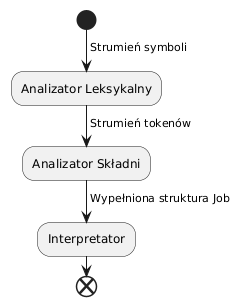
\includegraphics[width=0.4\textwidth]{Images/phases.png}
\end{figure}

Następnie opis procesu implementacji programu zostanie podzielony na części, które również dzielą się na fazy. Ma to na celu proste opisanie procesów zachodzących w środku programu, a także zademonstrowanie danych wejściowych/wyjściowych.

\section{Analiza}
Jak opisano powyżej, dane wejściowe są analizowane w części frontendowej programu. Analizator dzieli dane wejściowe na części i narzuca im strukturę gramatyczną, która później posłuży do zbudowania projektu. Jeżeli parser stwierdzi, że dane wejściowe są niepoprawne składniowo lub semantycznie, informuje o tym użytkownika w najbardziej zrozumiały sposób. Dodatkowo analizator zbiera informacje w postaci tablicy symboli, co zostanie opisane w dalszej części.

\subsection{Analiza leksykalna}
Analiza leksykalna jest pierwszym etapem analizy danych wejściowych. Analizator leksykalny odczytuje strumień symboli i grupuje je w sensowną sekwencję zwaną leksemami, dla których analizator leksykalny generuje tzw. token składający się z typu pary -- odwołanie do tabeli symboli \cite{compilers}.

W projekcie BBS analizator leksykalny jest podzielony na dwie odrębne klasy, \texttt{Lexer} i \texttt{Scanner}, dla których zaimplementowana jest także klasa pomocnicza \texttt{Context}. Także klasy te korzystają z dodatkowych elementów, które zostaną opisane później (ale będą tu omawiane tylko te, które naprawdę zasługują na uwagę, np. nie będzie tu opisu klas wyjątków).

\subsubsection{Klasa Scanner}
Klasa \texttt{Scanner} jest osobną klasą, której delegowana jest rola odczytu plików. To właśnie w tej klasie hermetyzowane są wszelkie operacje sprawdzania istnienia, otwierania i odczytywania plików znak po znaku, a także omijania pustych linii czy komentarzy. Jego implementacja jest dość prosta, gdyż \texttt{Scanner} umożliwia odczytanie bieżącego znaku (funkcja \texttt{Get()}) i przejście do następnego (funkcja \texttt{Move()}). Z kolei operacja \texttt{Get()} opiera się na \texttt{std::optional} \cite{cpp_optional}, innowacji w C++17, która pozwala przechowywać wartość lub nic w bezpieczny i przejrzysty sposób. Klasa na wejściu otrzymuje nazwę pliku do odczytania, a na wyjściu zwraca przeczytany znak (odfiltrowując niepotrzebne), jeśli takie istnieją.

Na szczególną uwagę zasługuje metoda o nazwie \texttt{Skip()} (wywoływana wewnątrz metody \texttt{Move()}), która wykonuje operację pomijania komentarzy i pustych znaków w przypadku konieczności przeczytania kolejnej linii (czyli oznacza, że został znaleziony znak nowej linii). Ta metoda wygląda następująco:

\begin{lstlisting}[label=list:scanner,caption=Metoda Scanner::Skip(),basicstyle=\footnotesize\ttfamily]
void Scanner::Skip()
{
    // Read the next line if scanner finds a new line symbol, a comment or an empty line
    auto character = context_.GetCharacter();
    while(!character || character.value() == constants::kComment)
    {
        std::string line;
        std::getline(file_, line);
        if(file_.fail())
        {
            file_.close();
            return;
        }
    
        context_.Update(std::move(line));
        character = context_.GetCharacter();
    }
    
    // Check if the line still has anything to read
    if(!character || character.value() == '\0')
    {
        file_.close();
    }
}
\end{lstlisting}

Analizując ten kod, możemy stwierdzić, że \texttt{Scanner} najpierw odczytuje bieżący znak, który następnie przechodzi sprawdzenie istnienia (\texttt{std::optional} jest pusty, jeśli znak nie był czytany przez zamknięty plik, np.) lub równość określonego w gramatyce języka symbolu komentarza. Następnie, w przypadku pozytywnego wyniku kontroli (pusty znak lub komentarz), \texttt{Scanner} próbuje odczytać następną linię. Jeśli instrukcja się powiedzie, \texttt{Scanner} aktualizuje kontekst nową linią i zapamiętuje nowy znak jako bieżący, po czym powtarzane jest sprawdzenie istnienia znaku lub komentarza (ponieważ nowa linia może zawierać także komentarz). Przy wyjściu z pętli \texttt{Scanner} sprawdza, czy ostatnia linia została odczytana i jeśli odpowiedź jest pozytywna, plik jest zamykany.

\subsubsection{Klasa Context}
Między innymi moduł \texttt{lexer} zawiera ważną klasę pomocniczą \texttt{Context}, której wpływ na moduł jest dość znaczący. Klasa ta pojawiła się w procesie rozbudowy i rozwoju projektu BBS poprzez wyodrębnienie metod i pól z klasy \texttt{Scanner} w celu nie tylko spełnienia zasad SOLID \cite{solid}, ale także ułatwienia dostępu do informacji o bieżącej lokalizacji w pliku. Funkcjonalność ta służy w szczególności szczegółowemu informowaniu użytkownika o błędach składniowych lub semantycznych.

Klasa \texttt{Context} zawiera bieżącą linię przetwarzaną przez program, jej indeks w pliku oraz pozycję bieżącego znaku w linii. Wszystkie pola są chronione i dostępne pośrednio poprzez predefiniowany interfejs.

\subsubsection{Klasa Lexer}
Klasa \texttt{Lexer}, jak sama nazwa wskazuje, jest implementacją analizatora leksykalnego. Ta klasa jest najbardziej złożona ze wszystkich w module, a jej struktura jest modułowa, co ułatwia zmianę jej elementów w miarę zmiany wymagań lub gramatyki języka.

Główna klasa \texttt{Lexer} ma tylko metody manipulacji tokenami (\texttt{Get()} do odczytania bieżącego tokena i \texttt{Next()} do żądania odczytania następnego tokena), ponieważ praca z plikami została delegowany do klasy \texttt{Scanner}.

Proces kategoryzacji tokenów został delegowany do szeregu klas zwanych procedurami obsługi. Klasy te stanowią implementację wzorca projektowego „Łańcuch odpowiedzialności” \cite{cor}, który polega na przetwarzaniu określonych żądań przez dany obiekt i ich późniejszym przekazywaniu do kolejnych obiektów, w przypadku gdyby żądanie nie powiodło się. Ten wzorzec został użyty, aby wycofać użycie \texttt{switch-case}, aby umożliwić znacznie łatwiejsze (i jednolite) podłączanie nowych klas obsługi przy minimalnych zmianach w istniejącym kodzie (zgodnie z zasadami SOLID \cite{solid}). Klasy te posiadają następujący interfejs:

\begin{lstlisting}[label=list:handler,caption=Klasa Handler,basicstyle=\footnotesize\ttfamily]
/**
 * @brief A default Lexer input handler, an implementation of the CoR pattern
 * 
 */
class Handler
{
    using Token = parser::tokens::Token;
    
public:
    /**
     * @brief Process the input and return the token if possible
     * 
     * @param scanner - the source of characters to process
     * @return std::unique_ptr<Token> - a pointer to the token or nullptr 
     */
    virtual std::unique_ptr<Token> Process(Scanner& scanner) const;
    
    /**
     * @brief Set the next handler to be called to process the input
     * 
     * @param next - a pointer to the next handler to be called
     */
    void SetNext(std::unique_ptr<Handler> next);
    
protected:
    /**
     * @brief A pointer to the handler, next on the line to process the input
     * 
     */
    std::unique_ptr<Handler> next_;
};
\end{lstlisting}

Oznacza to, że każdy obiekt przetwarzający po utworzeniu otrzymuje łącze do następcy, do którego zostanie przekazane żądanie w przypadku niepowodzenia podczas jego realizacji. Jeśli żaden z programów obsługi nie był w stanie przetworzyć żądania, ostatni w łańcuchu tworzy wyjątek. Implementacja ta pozwoliła maksymalnie uprościć klasę \texttt{Lexer}, kod metody \texttt{Next()}, która wymusza na parserze odczytanie kolejnego tokena z pliku, dzięki wzorcowi "łańcuch odpowiedzialności" \cite{cor} został uproszczony do następującej postaci bez poświęcania stabilności i bezpieczeństwa programu:

\begin{lstlisting}[label=list:scanner,caption=Metoda Lexer::Next(),basicstyle=\footnotesize\ttfamily]
std::shared_ptr<Lexer::Token> Lexer::Next()
{
    token_ = std::move(handler_->Process(scanner_));
    return token_;
}
\end{lstlisting}

Klasa \texttt{Lexer} na wejściu otrzymuje nazwę pliku (która jest przekazywana do obiektu klasy Scanner i nie jest zapisywana bezpośrednio), na wyjściu \texttt{Lexer} zwraca aktualny token, a także umożliwia odczytanie nowy. W przypadku znalezienia nieznanych symboli, których nie przewidywała gramatyka języka, analizator tworzy odpowiedni wyjątek ze szczegółowym opisem położenia symbolu i przyczyną błędu.

Lista tokenów, które program może przetworzyć, odpowiada podanemu językowi i została opisana w sekcji ''Gramatyk języka''.

\subsection{Analiza składni}

Po analizie leksykalnej lista tokenów wyodrębniona z plików wejściowych jest wysyłana do parsera. Praca parsera zazwyczaj polega na tworzeniu tzw drzewo składniowe, które jest pośrednią reprezentacją kodu wejściowego, odzwierciedlającą jego strukturę gramatyczną. Takie drzewo wygodnie zachowuje kolejność operacji i może wyglądać tak dla przykładowego wyrażenia $a = b + c$, gdzie $a$, $b$ i $c$ to identyfikatory dodane wcześniej do tablicy symboli:

\begin{lstlisting}[label=list:syntax_tree,caption=Struktura gramatyczna przykładowego wyrażenia,basicstyle=\footnotesize\ttfamily]
       =
     /	 \
<id, 1>   +
        /   \
   <id,2>   <id,3>
\end{lstlisting}

Jak wspomniano w sekcji ``Gramatyka języka'', opracowany język plików konfiguracyjnych projektu BBS jest dość prymitywny, co jest konsekwencją wymagań stawianych projektowi. Z tego powodu język nie obsługuje operacji arytmetycznych, łączenia ciągów znaków i zmiennych oraz nie zawiera żadnych innych typów danych niż typy „sekwencja znaków” i „tablica sekwencji znaków”. Biorąc pod uwagę wszystko, co napisano wcześniej, podjąłem decyzję o rezygnacji z implementacji parsera w taki sposób, aby możliwe było bezpośrednie utworzenie drzewa składniowego. Zamiast tego parser BBS, wykonując te same czynności, co wszystkie konwencjonalne parsery, natychmiast wykonuje funkcje zapisu danych projektu do pośredniej struktury danych.

Warto zaznaczyć, że parser ten stosuje podejście odgórne do analizy danych, czyli analizuje dane rozpoczynając od nieterminala początkowego i sprawdzając każdy symbol pod kątem zgodności z pochodnymi tego nieterminala. W przypadku BBS algorytm ten jest realizowany poprzez proste sprawdzenie danych wejściowych od lewej do prawej. Projektując spośród innych algorytmów (np. oddolnych) wybrano ten algorytm ze względu na prostotę implementacji, a także ze względu na ogólną prostotę zaimplementowanego języka.

Pełna funkcjonalność parsera w projekcie BBS zaimplementowana jest w klasach \texttt{Parser}, \texttt{Mediator}, a także klasach wywodzących się z interfejsu \texttt{State}.

\subsubsection{Tokeny}

Danymi wejściowymi dla parsera są ''tokeny'' -- sklasyfikowane dane, które odbierane są na wyjściu leksera. Program BBS dla ogólnej prostoty, co jest jednym z głównych wymagań, używa języka z tylko dwoma typami danych i praktycznie bez instrukcji. Poniżej znajduje się lista wszystkich tokenów, które mogą zostać przetworzone przez program BBS. Wykonanie każdego z nich jest podobne i bardzo proste, dlatego nie będzie tutaj opisywane.

\begin{itemize}
	\item \texttt{Operator} - ''='' oraz ''\$''
	\item \texttt{Punctuator} - kropki, przecinki, nawiasy oraz wykrzykniki
	\item \texttt{Separator} - spacje
	\item \texttt{Word} - litery alphabetu lacińskiego
\end{itemize}

\subsubsection{Klasa Parser}

Najważniejszą klasą jest klasa \texttt{Parser}, która w rzeczywistości jest implementacją wzorca projektowego ''State Machine'' \cite{state}. Ten wzorzec projektowy służy do przeniesienia każdego stanu klasy do osobnej klasy z własną implementacją tych samych metod. Decyzja o zastosowaniu tego szablonu wynikała z faktu, że parser jest maszyną stanową w klasycznym sensie, gdyż rolą parsera jest sprawdzanie tokenu po tokenie, przy czym każdy kolejny token jest całkowicie syntaktycznie zależny od poprzedniego (tj. jest jeden i sam token może być oczekiwany lub nieoczekiwany, w zależności od tokena, który był wcześniej przetwarzany przez parser).

Każdy stan parsera odpowiada oddzielnym nieterminalom zdefiniowanym w gramatyce języka użytego w projekcie. Interesująca jest implementacja każdego indywidualnego stanu, podczas gdy parser ma tylko jedną pełnoprawną metodę, która wywołuje metodę przetwarzania kolejnego znacznika bieżącego stanu i sprawdza istnienie tego stanu.


\begin{lstlisting}[label=list:parser,caption=Metoda Parser::Process(),basicstyle=\footnotesize\ttfamily]
scheduler::pipeline::Job Parser::Process()
{
    auto state = mediator_.GetState();
    while(state)
    {
        state->Process(lexer_);
    
        // Get the next state
        state = mediator_.GetState();
    }
    
    return mediator_.GetJob();
}
\end{lstlisting}

Każdy indywidualny stan implementuje wspólny dla wszystkich interfejs \texttt{State}, co zapewnia abstrakcję od szczegółów implementacji konkretnego stanu i znacznie upraszcza implementację samego parsera.

Ponadto ważnym elementem parsera jest także klasa \texttt{Mediator}, o czym będzie mowa później.

\subsubsection{Klasa Mediator}

Niezwykle ważną klasą jest klasa \texttt{Mediator}, która de facto jest implementacją znanego wzorca projektowego „Mediator”. Jego istotą jest uproszczenie połączeń pomiędzy klasami poprzez delegowanie metod komunikacji pomiędzy tymi klasami innej klasie zwanej ''Mediatorem'' \cite{mediator}.

W mojej implementacji parsera ta klasa jest potrzebna do uproszczenia zależności pomiędzy klasami \texttt{Parser}, każdą potomką interfejsów \texttt{State} i \texttt{Application}. Mediator ukrywa aktualny stan parsera, wskaźnik do obiektu struktury Job (o czym będzie mowa w następnej sekcji) oraz tablicę symboli. Wszystkie metody są w ten czy inny sposób getterami lub setterami, więc opisywanie ich implementacji nie jest tutaj szczególnie cenne.

\subsubsection{Klasy typów danych}

Jak już wspomniano, oprogramowanie to implementuje tylko dwa typy danych, a mianowicie „sekwencję znaków” i „tablicę sekwencji znaków”. Implementacja tych typów nie jest trudna i pod wieloma względami „tablica” opiera się na już istniejącej implementacji stanu „sekwencji znaków”, nie ma jednak pomiędzy nimi zależności hierarchicznych.

Każdy z tych typów implementuje interfejs \texttt{State}, co oznacza, że główną metodą, która nas interesuje w kontekście parsera jest \texttt{Process()}.

\begin{lstlisting}[label=list:string,caption=Metoda String::Process(),basicstyle=\footnotesize\ttfamily]
void String::Process(lexer::Lexer& lexer)
{
    // Skip separators in between the keyword and the
    auto token = State::SkipSeparators(lexer);

    // Expect the double quote mark at the start of the string
    Match(token.get(), ::parser::tokens::Punctuator::Type::kDoubleQuoteMark);
    
    // Add tokens one by one to the internal buffer
    while((token = lexer.Next()))
    {
        try
        {
            Match(token.get(), tokens::Punctuator::Type::kDoubleQuoteMark);
            return;
        }
        catch(const exceptions::UnexpectedTokenException&)
        {
            auto ptr = dynamic_cast<tokens::Operator*>(token.get());
            if(ptr && ptr->type == tokens::Operator::Type::kDollarSign)
            {
                Variable variable{mediator_};
                variable.Process(lexer);
    
                // Add variable's value to the result
                value_ += variable.GetValue();
    
                continue;
            }
    
            // Add the token to the whole value
            value_ += token->GetValue();
        }
    }
    
    throw exceptions::UnexpectedTokenException("");
}
\end{lstlisting}

Zacznijmy od przeanalizowania bardziej podstawowego typu ''sekwencji znaków''. Jak widać z powyższego kodu, każda sekwencja zaczyna się i kończy podwójnymi cudzysłowami, więc kod najpierw sprawdza, czy bieżący token jest cudzysłowem. Następnie każdy kolejny token (dowolnego typu) jest dodawany do wartości sekwencji, aż program napotka znak cudzysłowu. Jeśli token końcowy nie jest cudzysłowem, program zakończy działanie, zgłaszając wyjątek.

Na szczególną uwagę zasługuje ciąg znaków sprawdzający obecność znaku dolara, który reprezentuje nazwę zmiennej, co zostanie omówione w dalszej części tego rozdziału. Przed dodaniem tokena do pełnej wartości „ciągu znaków” parser sprawdza, czy nazwa zmiennej została odnaleziona. Jeżeli odpowiedź jest pozytywna, podejmowana jest próba zamiany nazwy zmiennej na jej wartość przy pomocy obiektu klasy \texttt{Variable}, który następnie jest dodawany do pełnej wartości ''ciągu znaków''


\begin{lstlisting}[label=list:array,caption=Metoda Array::Process(),basicstyle=\footnotesize\ttfamily]
void Array::Process(lexer::Lexer& lexer)
{
    // Skip separators in between the keyword and the
    auto token = SkipSeparators(lexer);

    // Expect the bracket at the start of the string
    Match(token.get(), tokens::Punctuator::Type::kLeftSquareBracket);

    // Process the tokens
    String string_handler{mediator_};
    do
    {
        // Get the next string
        string_handler.Process(lexer);
        value_.push_back(string_handler.GetValue());
        string_handler.Clear();

        // Get the terminator token
        token = SkipSeparators(lexer);

        // Try to match any punctuator
        try
        {
            Match(token.get(), tokens::Punctuator::Type::kRightSquareBracket);
            return;
        }
        catch(const exceptions::UnexpectedTokenException&)
        {
            Match(token.get(), tokens::Punctuator::Type::kComma);
        }
    } while(token);

    throw exceptions::UnexpectedEndOfFileException(lexer.GetContext());
}
\end{lstlisting}

Zamiast tego implementacja stanu \texttt{Array} jest bardziej złożona, ponieważ zamiast pojedynczego znaku kończącego, takiego jak cudzysłowy w ciągu znaków, tablica używa przecinków do oddzielania kolejnych sekwencji znaków, a także nawiasów kwadratowych aby zaznaczyć krawędzie tablicy. Zamiast tego w kodzie przetwarzającym ciągi znaków wykorzystano gotową klasę \texttt{String}, co znacznie upraszcza implementację tablic oraz poprawia jakość, stabilność i czystość kodu.

\subsubsection{Klasy słów kluczowych}

Implementacja każdego słowa kluczowego wymagała oddzielnych klas, ale w rzeczywistości wszystkie z nich są potomkami klas \texttt{String} lub \texttt{Array} (w zależności od cech gramatycznych konkretnego słowa). Podobnie jak omówione powyżej klasy typu bazowego, klasy każdego pojedynczego słowa posiadają własną implementację metody \texttt{Process()}, która służy do przetwarzania tokenów otrzymanych od obiektu klasy \texttt{Lexer}. Wszystkie słowa są opisane w sekcji ''Gramatyka języka''.

Przykładem słowa kluczowego wywodzącego się z typu „sekwencja znaków” jest \texttt{cflags}, czyli słowo definiujące parametry kompilacji projektu. Jak widać z poniższego kodu, w metodzie \texttt{Process} odpowiedniej klasy najpierw wykonywana jest metoda klasy nadrzędnej, a następnie wynikowa wartość przekazywana jest do obiektu klasy \texttt{Job} poprzez odpowiednie wywołanie metody. Sam obiekt uzyskuje się poprzez wywołanie modułu pobierającego obiekt mediatora. Ostatnim krokiem jest przejście do stanu standardowego \texttt{Statement}, który rozpoczyna cykl przetwarzania każdej linii od nowa (zgodnie z architekturą odgórną parsera).

\begin{lstlisting}[label=list:cflags,caption=Metoda CFlags::Process(),basicstyle=\footnotesize\ttfamily]
void CFlags::Process(lexer::Lexer& lexer)
{
    String::Process(lexer);

    // Set the compilation flags
    auto& job = mediator_.BorrowJob();
    job.SetCompilationFlags(std::move(GetValue()));

    // Return to the Statement state
    mediator_.SetState(std::make_unique<Statement>(mediator_));
}
\end{lstlisting}
    
Na szczególną uwagę zasługuje klasa \texttt{Keyword}, która jest implementacją stanu parsera odpowiadającego nieterminalowi o tej samej nazwie. Jej celem jest przejście do prawidłowego stanu słowa kluczowego w celu jego obsługi przez program, metoda \texttt{Process()} tej klasy jest niczym innym jak implementacją wzorca projektowego ''Metoda fabryczna'' [link] , wzór generujący. Metoda ta ma konstrukcję \texttt{switch-case} i nie różni się niczym innym.

\begin{lstlisting}[label=list:keywords,caption=Metoda Keyword::Process(),basicstyle=\footnotesize\ttfamily]
void Keyword::Process(lexer::Lexer& lexer)
{
    // Check if the next token exists
    const auto token = lexer.Next();
    if(!token)
    {
        throw exceptions::UnexpectedEndOfFileException(lexer.GetContext());
    }

    // Process the correct keyword
    const auto& keyword = token->GetValue();
    if(keyword == "cflags")
    {
        mediator_.SetState(std::make_unique<keywords::CFlags>(mediator_));
        return;
    }
    else if(keyword == "deps")
    {
        mediator_.SetState(std::make_unique<keywords::Deps>(mediator_));
        return;
    }
    else if(keyword == "files")
    {
        mediator_.SetState(std::make_unique<keywords::Files>(mediator_));
        return;
    }
    else if(keyword == "prj")
    {
        mediator_.SetState(std::make_unique<keywords::Project>(mediator_));
        return;
    }
    else if(keyword == "pre")
    {
        mediator_.SetState(std::make_unique<keywords::Pre>(mediator_));
        return;
    }
    else if(keyword == "post")
    {
        mediator_.SetState(std::make_unique<keywords::Post>(mediator_));
        return;
    }
    else if(keyword == "let")
    {
        mediator_.SetState(std::make_unique<keywords::Let>(mediator_));
        return;
    }
    else if(keyword == "inc")
    {
        mediator_.SetState(std::make_unique<keywords::Inc>(mediator_));
        return;
    }
    
    throw exceptions::UnexpectedKeywordException(lexer.GetContext(), token->GetValue());
}
\end{lstlisting}

\subsubsection{Klasa Variable}

Jedną z najważniejszych klas stanu i filarem funkcji wykorzystania i przetwarzania zmiennych języka projektu jest klasa \texttt{Variable}. Klasa ta zajmuje się wyłącznie przetwarzaniem nazw zmiennych i na wyjściu zwraca wartość tej zmiennej, jeśli została ona wcześniej dodana do tablicy symboli.

Implementacja tej klasy nie jest zbyt trudna, nie jest podobna do żadnej innej metody pokrewnych klas i opiera się w dużej mierze na obiekcie Mediator, który sam ma tablicę symboli.

\begin{lstlisting}[label=list:keywords,caption=Metoda Keyword::Process(),basicstyle=\footnotesize\ttfamily]
void Variable::Process(lexer::Lexer& lexer)
{
    // Check if EOF is reached
    const auto token = lexer.Next();
    if(!token)
    {
        throw exceptions::UnexpectedEndOfFileException(lexer.GetContext());
    }

    // Check if the ID is a word
    auto ptr = dynamic_cast<tokens::Word*>(token.get());
    if(!ptr)
    {
        throw exceptions::UnexpectedTokenException(token->GetValue());
    }
    
    value_ = mediator_.GetVariableValue(token->GetValue());
}
\end{lstlisting}

Jak widać z implementacji głównej metody klasy powyżej, pierwszym etapem jej pracy jest pobranie i sprawdzenie aktualnego tokena pod kątem poprawności (nazwa zmiennej może być tylko słowem, w odróżnieniu od typu „sekwencja znaków”, który może zaakceptować prawie wszystko). Po wszystkich niezbędnych sprawdzeniach metoda zwraca wartość zmiennej, jeśli taka istnieje.

\subsubsection{Klasa Statement}

Ta klasa jest nieterminalną implementacją o tej samej nazwie. Ta klasa jest wyłącznie odpowiedzialna za sprawdzanie obecności wykrzyknika na początku każdego słowa kluczowego i przejście do stanu „Słowo kluczowe”.

\subsubsection{Klasa State}

Klasa \texttt{State} stanowi interfejs dla wszystkich klas stanu parsera, dzięki czemu już na etapie parsowania osiągana jest poprawna i wydajna architektura projektu. Jednak dodatkowo klasa ta zawiera bez przesady najważniejsze metody dla wszystkich stanów, a mianowicie

\begin{itemize}
	\item SkipSeparators() - odpowiada za pomijanie znaków oddzielających
	\item Match() - sprawdzanie typu interpunkcji pod kątem równości z bieżącym tokenem
\end{itemize}

Implementacja metody SkipSeparators() polega na odebraniu kolejnych tokenów z obiektu klasy \texttt{Lexer} i próbie ich skonwertowania do typu \texttt{Separator}. Pierwszy token nieseparator opuszcza pętlę i kończy funkcję.

\begin{lstlisting}[label=list:separator_skip,caption=Metoda State::SkipSeparators(),basicstyle=\footnotesize\ttfamily]
std::shared_ptr<tokens::Token> State::SkipSeparators(lexer::Lexer& lexer)
{
    std::shared_ptr<tokens::Token> token;
    while((token = lexer.Next()))
    {
        // Token might be nullptr, handle this case
        if(!token)
        {
            throw std::runtime_error("State::SkipSeparators() was called with nullptr.");
        }
    
        if(!dynamic_cast<tokens::Separator*>(token.get()))
        {
            break;
        }
    }
    
    return token;
}
\end{lstlisting}

Z kolei metoda \texttt{Match()} działa podobnie jak poprzednia: jej zasada polega na konwersji wskaźnika na token na typ \texttt{Punctuator}, który następnie jest sprawdzany pod kątem identyczności z żądanym.

\begin{lstlisting}[label=list:match,caption=Metoda State::Match(),basicstyle=\footnotesize\ttfamily]
void State::Match(tokens::Token* token, tokens::Punctuator::Type value)
{
    if(!token)
    {
        throw exceptions::UnexpectedTokenException("EOF");
    }
    
    const auto ptr = dynamic_cast<tokens::Punctuator*>(token);
    if(!ptr || ptr->type != value)
    {
        throw exceptions::UnexpectedTokenException(std::move(token->GetValue()));
    }
}
\end{lstlisting}

\subsection{Analiza semantyczna}

Analizator semantyczny wykorzystuje drzewo składni i informacje zawarte w tablicy symboli, aby sprawdzić program źródłowy pod kątem zgodności semantycznej z definicją języka. Gromadzi również informacje o typie i przechowuje je w drzewie składni lub tabeli symboli do późniejszego wykorzystania podczas pośredniego generowania kodu.
Na przykład wiele zdefiniowanych języków programowania wymaga, aby indeks tablicy był liczbą całkowitą; kompilator powinien zgłosić błąd, jeśli do indeksowania tablicy użyto liczby zmiennoprzecinkowej.

Ponieważ program BBS nie musi generować żadnego kodu (tj. nie jest kompilatorem), co oznacza, że nie musi generować drzewa składniowego, nie zaimplementowano etapu analizy semantycznej. Decyzja ta ilustruje także fakt, że początkowy wymóg nałożył duże ograniczenie na liczbę typów danych wewnętrznych sprawdzanych przez usługę BBS, a także typów, które nie wymagają odpowiedniej konwersji czy adresowania tablic. Podsumowując, analiza semantyczna nie stała się częścią programu BBS.
